\section{Projekt Valhalla}\label{sec:valhalla}

Das OpenJDK-Projekt \emph{Valhalla}~\cite{openjdk-valhalla} besteht aus drei wesentlichen Neuerungen, die in folgenden \acp{jep} definiert sind:

\begin{itemize}
    \item \ac{jep} 169: Value Objects~\cite{jep-169}
    \item \ac{jep} 193: Variable Handles~\cite{jep-193}
    \item \ac{jep} 218: Generics over Primitive Types~\cite{jep-218}
\end{itemize}

Grundlage für die Änderungen des Projekts stellen die \emph{Value Objects} dar.
Deren Ziel ist es, die \ac{jvm} mit Unterstützung für neue benutzerdefinierbare Typen zu erweitern, die im Vergleich zu bestehenden Klassen keine Referenzsemantik haben, sondern sich wie primitive Datentypen verhalten.
Unterabschnitt~\ref{subsec:value-types} erläutert diese näher.

Die \emph{Variable Handles} bezeichnen einen Teil der Java Standard-Bibliothek, die präziseren Zugriff auf Felder von Objekten und Array-Elementen ermöglichen.
Sie erlaubt unter Anderem die Kontrolle der Zugriffsreihenfolge durch mehrere Threads. % TODO can be removed
Die Implementierung der API erfolgte bereits in Java 9 und wird daher nicht näher in dieser Arbeit betrachtet.

Die Erweiterung von generischen Typen mit Unterstützung für primitive Typen ist der größte Teil des Projekts.
Sie verlangt weitreichende Änderungen, die sowohl die Sprache als auch die \ac{jvm} betreffen.
In Unterabschnitt~\ref{subsec:primitive-generics} erfolgt eine Vertiefung in dieses Thema.

\subsection{Value Types}\label{subsec:value-types}

Seit der ersten Version von Java im Jahr 1995 verfolgt die Programmiersprache den Ansatz, dass alles außer primitive Werte ein Objekt ist.
Das unterscheided Java von Programmiersprachen wie C oder C++, wo primitive Werte sowie durch Klassen und Structs definierte Aggregate davon zunächst nur einfache Werte sind und erst durch Pointer eine Referenzsemantik erhalten.

In Java sind hingegen alle Variablen und Parameter vom Typ einer Klasse implizit Pointer.
Dies vereinfacht das Programmiermodell und ist weniger fehleranfällig, besonders durch die Präsenz des Garbage Collectors.
Es führt jedoch auch dazu, dass alle Zugriffe auf Daten in diesen Objekten über Indirektion erfolgen.
Dies verringert die Lokalität der Daten und führt auf heutiger Hardware, auf der Zugriffe auf den Hauptspeicher wesentlich länger dauern als auf den CPU-Cache-Speicher, zu deutlich langsamerer Performance. % TODO ww führt
Weiterhin erzeugen Referenzen einen deutlichen höheren Speicherverbrauch, wie ein Beispiel zeigen wird. % TODO wo?
Zuletzt sorgt die Allokation und Freigabe des Speichers, besonders bei einer Vielzahl kleiner Objekte, für einen Verwaltungsaufwand seitens des Allocators und Garbage Collectors.

Aufgrund dieser Performance-\ und Speicherbedenken suchen viele Java-Entwickler nach Möglichkeiten, Klassen und Objekte zu umgehen.
Meist entsteht dabei Code, der händische Optimierungen auf Kosten von Lesbarkeit, Abstraktion und Fehlersicherheit enthält.
Value Types sollen dies vermeiden.

% Unterschiede zu Referenzen, Pointerfreiheit
Es soll nun betrachtet werden, was Value Types von regulären Referenztypen unterscheided.
Größter Unterschied ist die \emph{Pointerfreiheit}.
Ohne Pointer funktionieren einige Konzepte nicht mehr, die bisher alltäglich waren.
So besitzen Werte keine Identität mehr, die verglichen werden könnte, und damit auch keinen Identitäts-Hashcode.
Weiterhin können sie nicht mehr als Monitor dienen, da ohnehin nicht von zwei Threads darauf zugegriffen werden kann.
Die \code{clone}-Operation ist nicht mehr sinnvoll, ebenso der Finalizer, da die Werte nicht mehr vom Garbage Collector verarbeitet werden.
Auch \code{null} ist kein gültiger Wert mehr, allerdings wäre eine Alternative möglich, die den Speicher für den Wert auf null setzt.
Zuletzt kann nicht von Value Types geerbt werden, da im Voraus bekannt sein muss, wie viel Speicherplatz reserviert werden muss, was mit Vererbung nicht statisch entschieden werden könnte.
Veränderungen der Felder von Werten würde sich nur auf die lokale Kopie auswirken, wie es bereits von primitiven Typen bekannt ist.
Die Veränderung von \code{this} in Methoden eines Value Types ist folglich nicht mehr sinnvoll, wodurch Seiteneffekte vermieden werden und nachvollziehbarer Code entsteht.

% TODO Ziel von Value Types

% Memory example
Um das Speicherproblem näher zu erläutern, soll nun ein Beispiel betrachtet werden.
Es sollen einige ganzzahlige Punkte im zweidimensionalen Raum gespeichert die einen Pfad bilden.
Die Punkte sind als Objekte mit zwei \code{int}-Feldern modelliert, der Pfad als Array von Punkten.
Bei einer Pfadlänge von drei berechnet sich der Speicherverbrauch wie folgt:

\[ \SI{24}{\byte} \text{(Array-Header)} + 3 \cdot \SI{8}{\byte} \text{(Referenzen im Array)} + 3 \cdot (\SI{16}{\byte} \text{(Objekt-Header)} + 2 \cdot \SI{4}{\byte} \text{(int-Werte)}) = \SI{120}{\byte} \]

Ein Objekt, das zwei \code{int}-Werte beeinhaltet, benötigt auf einer 64-bit \ac{jvm} $\SI{8}{\byte}$ für die Referenz selber, $\SI{16}{\byte}$\footnote{Mit \code{-XX:+UseCompressedOops} könnte dies auf $\SI{12}{\byte}$ reduziert werden, allerdings kommen dann $\SI{4}{\byte}$ Padding hinzu, da die Größere von Objekten im Heap ein Vielfaches von $\SI{8}{\byte}$ sein muss.} für den Objekt-Header und je $\SI{4}{\byte}$ für die beiden \code{int}-Werte.
Die Größe eines Array-Headers beträgt $\SI{24}{\byte}$.
Mit drei Objekten ergibt sich also insgesamt ein Speicherverbrauch von $\SI{120}{\byte}$.

Das gleiche Beispiel soll nun mit Value-Typen realisiert werden.
Dabei entfallen die Objekt-Header und Referenzen vollständig.
Der neue Speicherverbrauch berechnet sich also wie folgt:

\[ \SI{24}{\byte} \text{(Array-Header)} + 3 \cdot 2 \cdot \SI{4}{\byte} \text{(int-Werte)} = \SI{48}{\byte} \]

Folglich konnten $\SI{72}{\byte}$ eingespart werden.
Zu beachten ist auch, dass die gesamten Daten des Arrays mit einer Größe von $\SI{48}{\byte}$ in eine Cache-Zeile passen, wenn bei deren Größe von $\SI{64}{\byte}$ ausgangen wird.
Der Effekt wird verstärkt, wenn das Array mehr Elemente enthält.

In Abbildung~\ref{fig:memory-usage} erfolgt eine grafische Darstellung des verringerten Speicherverbrauchs.
Sie zeigt links das Speicherlayout in heutigen \acp{jvm} und rechts das Speicherlayout, wenn Value Types für die Punkte verwendet werden.
Die Höhe der Rechtecke mit Zahlen entspricht hier $\SI{4}{\byte}$.

\begin{figure}
    \centering
    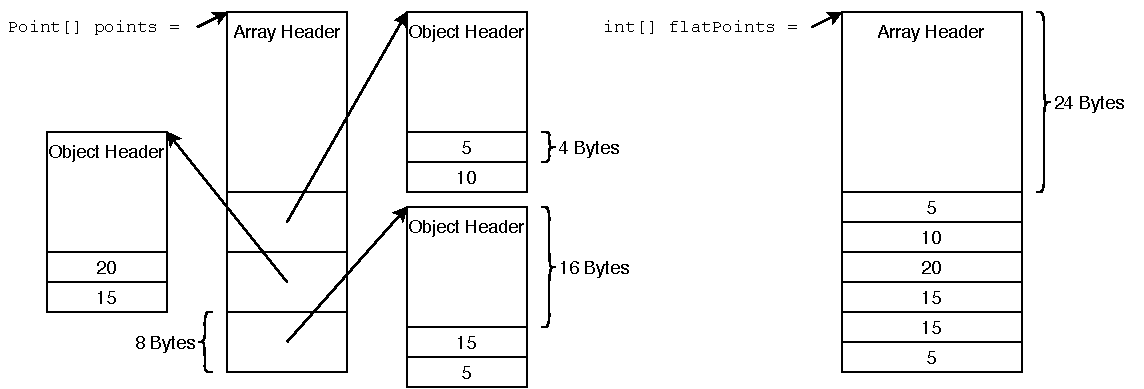
\includegraphics{img/memory-usage.pdf}
    \caption{Vergleich des Speicherlayouts eines Arrays von Punkten heute und mit Value Types}
    \label{fig:memory-usage}
\end{figure}

\subsection{Primitive und generische Typen}\label{subsec:primitive-generics}
